\documentclass{llncs}

%\usepackage{times}
\usepackage[utf8]{inputenc}
\usepackage{amsfonts}
%\usepackage{qtree}
\usepackage{xspace}

%\usepackage{makeidx}  % allows for indexgeneration
%\usepackage{graphicx,times,psfig,amsmath} % Add all your packages here
%\usepackage{hyperref}
\usepackage{amsmath}
%\usepackage{amssymb}
\usepackage{graphicx}

\usepackage[ampersand]{easylist}
\usepackage[usenames,dvipsnames]{color}

\newcommand{\Lets}{Let us\xspace}
\newcommand{\lets}{let us\xspace}
\newcommand{\lterm}{$\lambda$-term\xspace}
\newcommand{\lterms}{$\lambda$-terms\xspace}
\newcommand{\lhead}{$\lambda$-head\xspace}
\newcommand{\lheads}{$\lambda$-heads\xspace}
\newcommand{\la}{\leftarrow\xspace}
\newcommand{\Lp}  {\Lambda^{\prime}\xspace}
\newcommand{\tur}[3]{#1\vdash{}#2 \colon #3}
\newcommand{\turst}[3]{$#1\vdash{}#2:#3$\xspace}
\newcommand{\GMS}{\turst{\Gamma}{M}{\sigma}}
\newcommand{\atTree}{@-tree\xspace}
\newcommand{\setDots}[2]{ \lbrace #1 , \dots , #2 \rbrace}
\newcommand{\lh}[1]{\lambda #1}
\newcommand{\sexprTree}{sexpr-tree\xspace}
\newcommand{\SexprTree}{Sexpr-tree\xspace}
\newcommand{\then}{\Rightarrow\xspace}
\newcommand{\lamb}[2]{( \lambda \, #1 \, . \, #2 )}
\newcommand{\lam}[2]{\lambda \, #1 \, . \, #2}
\newcommand{\ST}{\mathop{\mathrm{ST}}}
\newcommand{\FV}{\mathop{\mathrm{FV}}}
\newcommand{\Scomb }{\mathbf{S}}
\newcommand{\Kcomb }{\mathbf{K}}
\newcommand{\Icomb }{\mathbf{I}}
\newcommand{\bbarr}{\twoheadrightarrow_\beta}
\newcommand{\barr}{\rightarrow_\beta}
\newcommand{\beq}{=_\beta}
\newcommand{\eearr}{\twoheadrightarrow_\eta}
\newcommand{\earr}{\rightarrow_\eta}
\newcommand{\eeq}{=_\eta}
\newcommand{\bearr}{\rightarrow_{\beta\eta}}
\newcommand{\bbeearr}{\twoheadrightarrow_{\beta\eta}}
\newcommand{\beeq}{=_{\beta\eta}}
\newcommand{\etar}{\twoheadrightarrow_\eta}
\newcommand{\ered}{$\eta$-reduction\xspace}
\newcommand{\bnf}{$\beta$-\textit{nf}\xspace}
\newcommand{\enf}{$\eta$-\textit{nf}\xspace}
\newcommand{\eenf}{$\eta^{-1}$-\textit{nf}\xspace}
\newcommand{\beenf}{$\beta\eta^{-1}$-\textit{nf}\xspace}
\newcommand{\benf}{$\beta\eta$-\textit{nf}\xspace}
\newcommand{\bredex}{$\beta$-redex\xspace} 
\newcommand{\lnf}{\textit{lnf}\xspace}
\newcommand{\Ae}{\mathop{\mathrm{\AE}}}
\newcommand{\Bcomb }{\mathbf{B}}   
\newcommand{\BBcomb }{\mathbf{B*}}
\newcommand{\Ccomb }{\mathbf{C}}   
\newcommand{\CCcomb }{\mathbf{C'}}
\newcommand{\SScomb }{\mathbf{S'}}
\newcommand{\ar}{\rightarrow\xspace}
\newcommand{\T}{\mathbb{T}\xspace}
\newcommand{\C}{\mathbb{C}\xspace}
\newcommand{\Real}{\mathbb{R}}

\newenvironment{todo}
{~\\ {\color{red}\textbf{TODO}}
  \begin{easylist}[itemize]}
{ \end{easylist}}

\newcommand{\Lpr}{\Lambda^\prime}
\newcommand{\ul}[2]{\langle #1 ; #2 \rangle}
\newcommand{\ro}[1]{{\color{blue} #1}}
\newcommand{\tom}[1]{{\color{ForestGreen} #1}}
\newcommand{\red}[1]{{\color{red} #1}}

%\hyphenation{op-tical net-works semi-conduc-tor IEEEtran}

\begin{document}

\title{
Generating Lambda Term Individuals in Typed Genetic Programming Using Forgetful A*}
%\author{Tom\'{a}\v{s} K\v{r}en\inst{1} \and Roman Neruda\inst{2}}
%\institute{%
%Faculty of Mathematics and Physics\\
%Charles University in Prague\\
%Malostransk\'e n\'am\v{e}st\'\i~25, 11000 Prague, Czech Republic\\
%\email{tomas.kren@mff.cuni.cz}
%\and
%Institute of Computer Science\\
%Academy of Sciences of the Czech Republic\\
%Pod Vod\'arenskou v\v{e}\v{z}\'\i~2, 18207, Prague, Czech Republic\\
%\email{roman@cs.cas.cz}
%}
\maketitle

\begin{abstract}
In this paper, a generalization of genetic programming 
for simply typed lambda calculus is presented. We propose three population 
initialization methods depending on different search strategies. 
The first strategy corresponds to standard ramped half-and-half initialization, 
the second one corresponds to exhaustive systematic search, and the third one 
represents a novel geometric strategy. Three well-known benchmark experiments
support that the geometric strategy outperforms
the standard generating method in success rate, time consumption and average individual size. 
%Other performance enhancements based on theory of lambda calculus are 
%proposed and supported by experiments, including abstraction elimination 
%that enables us to utilize a simple tree-swapping crossover.
\end{abstract}


\section{Introduction}

%\subsection{gp a typy jsou dobrý / motivace}
%...
%\subsection{příběh}

%(...)\\


Genetic programming (GP) represents an efficient method for automatic generating of programs by means of evolutionary techniques~\cite{koza92,koza03}. Early attempts to enhance the GP approach with the concept of types include the seminal work~\cite{montana95} where the ideas from Ada programming language were used to define a so-called strongly typed GP.   
Use of types naturally opens door to enriching S-expressions,
the traditional GP representation of individuals, with concepts from
lambda calculus, which is simple yet powerful functional mathematical and programming 
language extensively used in type theory. Such attempts has shown to be 
successful \cite{yu01}. 

The key issue in the lambda calculus approach to enrich GP with types is the method of individual generation. During the expansion phase the set of unfinished terms can be browsed with respect to various search strategies. Our approach to this problem aims to utilize the full arsenal given by the simply typed lambda calculus. Thus, the natural idea is to employ an exhaustive systematic search. On the other hand, if we were to mimic the standard GP approach, a quite arbitrary yet common and successful ramped half-and-half generating heuristic~\cite{fg} should probably be used.  
These two search methods in fact represent boundaries between which we will try to position our parameterized solution that allows us to take advantage of both strategies. This design goal also differentiate our approach from 
the three state of the art proposals for typed GP known to us that are discussed in the following section. 
Our proposed \emph{geometrical search strategy} described in this paper is such a successful hybrid mixture of random and systematic exhaustive search. Experiments show that it is also very efficient dealing with one of the traditional GP scarecrows - the bloat problem.


%~\\(...)
%
%~\\
%\textbf{poznamky naky}\textit{\\
%- geometrická strategie generování termů jakožto hybrid systematického a náhodného sytylu --- to že jsme si vytičili ty dva cíle který plníme tou 
%jednoduchou strategií, tak máme možnost nalízt jednoduchou strategii která 
%je na pomezí obou cílů - taková strategie je právě ta naše geometrická 
%a ukazuje se že se bohulibě chová právě k strašáku GP -- \textbf{bloatu}.\\
%- teoretické LC konstrukty s výhodou použity - @-stromy a eta-redukce\\
%- křížení by eliminace 
%}

%\subsection{obsah kapitol článku v 1 větě}

The rest of the paper is organized as follows: The next section briefly discusses related work in the field of typed GP, while section~\ref{preliminaries} introduces necessary notions. Main original results about search strategies in individual generating are described in section~\ref{approach}. Section~\ref{experiments} presents results of our method on three well-known tasks, and the paper is concluded by section~\ref{conclusions}.

\section{Related work}
\label{related}


In \cite{yu01} Yu presents a GP system utilizing
polymorphic higher-order functions\footnote{Higher-order 
function is a function taking another function as 
input parameter.} and lambda abstractions.
Important point of interest in this work is use of
\texttt{foldr} function as a tool for \textit{implicit recursion},
i.e. recursion without explicit recursive calls. 
The terminal set for constructing lambda abstraction subtrees 
is limited to use only constants and variables of that particular
lambda abstraction, i.e., outer variables are not allowed to be used
as terminals in this work. This is significant difference from our approach 
since we permit all well-typed normalized \lterms. From this difference also
comes different crossover operation. We focus more on term generating process; 
their term generation is performed in a similar way as the standard one, 
whereas our term generation also tries to utilize techniques of systematic enumeration. 

In \cite{kes} Briggs and O’Neill present technique 
utilizing typed GP with combinators.
The difference between approach presented in this work
and our approach is that in this work terms are generated
straight from \textit{library} of combinators and no lambda abstractions
are used. They are using more general polymorphic type system then us
-- the Hindley–Milner type system. They also discuss the 
properties of exhaustive enumeration of terms and compare it with GP search.  
They also present interesting concept of \textit{Generalized
genetic operator} based on term generation. 

In \cite{binard2008genetic} by Binard and Felty even 
stronger type system (\textit{System F}) is used.  
But with increasing power of the type system comes increasing difficulty of term generation.
For this reason evolution in this work takes interesting and nonstandard shape 
(fitness is associated with \textit{genes} which are evolved together with \textit{species}
which together participate in creation of individuals).
This differs from our approach, which tries to be generalization of
the standard GP\cite{koza92}.

In contrast with above mentioned works our approach uses very simple type system 
(simply typed lambda calculus) and concentrates on process of generation  
able to generate all possible well-typed normalized lambda terms. In order to do
so we use technique based on \textit{inhabitation machines} 
described by Barendregt in~\cite{barendregt10}.    

\section{Preliminaries}
\label{preliminaries}
%definice, pojmy
%\subsection{Term}

In this section, several notions necessary to build a typed GP based on lambda calculus are introduced. 
First, \lets 
%Here we  %formally 
describe a programming language, 
in which the GP algorithm generates individual programs --- the so called \lterms.  


\begin{definition}
Let $V$ be infinite countable set of {\it 
variable names}. Let $C$ be set of {\it constant names}, 
$V \cap C = \emptyset$.	 	
Then $\Lambda$ is set of {\it \lterms} defined inductively as follows.	
\begin{align*}
x   \in V \cup C  &\then x     \in \Lambda \\
M,N \in \Lambda   &\then (M~N) \in \Lambda 
\textit{~~~~~~(Function application)} \\
x   \in V , M \in \Lambda &\then \lamb{x}{M} \in \Lambda
\textit{~~~~($\lambda$-abstraction)} 
\end{align*}
\end{definition}

\textit{Function application} and 
\textit{$\lambda$-abstraction} are concepts
well known from common programming languages. 
For example in JavaScript 
$(M~N)$ translates to expression \texttt{$M$($N$)} and
$\lamb{x}{M}$ translates to expression \texttt{function($x$)\{return $M$;\}}.
In other words, the function application 
corresponds to the act of supplying a function 
with an argument, and
the $\lambda$-abstraction is equivalent to 
\textit{anonymous function}\footnote{Apart from JavaScript, anonymous functions are common e.g. in Python and Ruby, 
they were recently introduced to C++, and they are expected to be supported in Java 8.}.
$M_1~M_2~M_3~\dots~M_n$ is an abbreviation for $(\dots((M_1~M_2)~M_3)~\dots~M_n)$
and $\lam{x_1 x_2 \dots x_n }{M}$ for $\lamb{x_1}{\lamb{x_2}{\dots\lamb{x_n}{M}\dots}}$.

%\subsubsection{Reductions}
%(... zmiňovat ? a pokud ano tak tady nebo radši v sekci která diskutuje 
%normálnost vygenerovanejch termů a jejich zkrácení pomocí $eta$-redukce)
%\subsubsection{Tree representations}
%(... zmiňovat ?)
%\subsection{Type}

A \lterm as described above
corresponds to a program expression with no type information
included. Now we will describe \textit{types} (or \textit{type terms}).

\begin{definition}
Let $A$ be set of {\it atomic type names}. 
Then $\mathbb{T}$ is set of {\it types} inductively defined as follows.
\begin{align*}
\alpha      \in A  &\then   \alpha \in \T \\
\sigma,\tau \in \T &\then ( \sigma \ar  \tau ) \in \T 
\end{align*}
\end{definition}

Type $\sigma \ar \tau$ is type for functions taking as input
something of a type $\sigma$ and returning 
as output something of a type $\tau$. 
$\tau_1 \ar \tau_2 \ar \dots \ar \tau_n$ is an abbreviation for 
$\tau_1 \ar (\tau_2 \ar (\dots \ar (\tau_{n-1} \ar \tau_n)\dots))$.
The system called \textit{simply typed $\lambda$-calculus} is now easily obtained by
combining the previously defined \textit{\lterms} and \textit{types} together. 


%\subsection{Context}



\begin{definition}\begin{enumerate}
 \item 	Let $\Lambda$ be set of {\it \lterms}. 
	Let $\mathbb{T}$ be set of {\it types}.       
	A {\it statement} $M : \sigma$ is a pair 
	$(M,\sigma) \in \Lambda \times \mathbb{T}$.
	Statement $M : \sigma$ is vocalized as 
	{\it "$M$ has type $\sigma$"}.
	The term $M$ is called the {\it subject} of the 
	statement $M : \sigma$.
 \item A \textit{declaration} is a statement 
 $x : \sigma$ where $x \in V \cup C$.
  
 \item A \textit{context} 
 %(or \textit{basis}) 
 is set of declarations with distinct variables as subjects.
\end{enumerate}
\end{definition}

Context is a basic type theoretic concept suitable as a typed alternative
for terminal and function set in standard GP. 
Notation $\Gamma,x:\sigma $ denotes $ \Gamma\cup\{(x:\sigma)\}$ 
such that $\Gamma$ does not contain any declaration with $x$ as subject.
We also write $x:\sigma \in \Gamma$ instead of $(x,\sigma) \in \Gamma$.


%\subsection{Simply typed $\lambda$-calculus}

\begin{definition}
A statement $M\colon\sigma$ is \textit{derivable from}
a context $\Gamma$ (notation 
\mbox{$\Gamma\vdash{}M\colon\sigma$}) 
if it can be produced by the following rules.
\begin{align*}
x : \sigma \in \Gamma &~\then~ \tur{\Gamma}{x}{\sigma}\\
\tur{\Gamma}{M}{\sigma \ar \tau}~,~\tur{\Gamma}{N}{\sigma} 
&~\then~ \tur{\Gamma}{(M~N)}{\tau}\\  
\tur{\Gamma,x:\sigma}{M}{\tau}
&~\then~ \tur{\Gamma}{\lamb{x}{M}}{\sigma \ar \tau} 
\end{align*}
\end{definition}

Our goal in term generation is to produce terms $M$
for a given pair $\ul{\tau}{\Gamma}$
such that for each $M$ is $\tur{\Gamma}{M}{\tau}$.




%\begin{todo}
%    & From this definition we can derive following rules...
%
%	& citovat něco, asi barendrechta 
%	(on to tam ale nějak moc nedokazuje) 
%	případně mojí diplomku (tam to dokazuju)
%\end{todo}

%\subsection{Unfinished term}

\begin{definition}
Let $V$ be infinite countable set of {\it 
variable names}. Let $C$ be set of {\it constant names}, 
$V \cap C = \emptyset$.	
Let $\T$ be set of types.
Let $\C$ be set of all contexts on ($V \cup C$, $\T$).
Then $\Lpr$ is set of 
\textit{unfinished  \lterms} defined inductively as follows.	
\begin{align*}
\tau \in \T , \Gamma \in \C &\then \ul{\tau}{\Gamma} \in \Lpr
\textit{~~~~~~~~(Unfinished leaf)}\\
x   \in V \cup C  &\then x     \in \Lpr \\
M,N \in \Lpr   &\then (M~N) \in \Lpr 
\textit{~~~~~~(Function application)} \\
x   \in V , M \in \Lpr &\then \lamb{x}{M} \in \Lpr
\textit{~~~~($\lambda$-abstraction)} 
\end{align*}
\end{definition}

\textit{Unfinished leaf} $\ul{\tau}{\Gamma}$ 
stands for yet not specified \lterm of the type $\tau$ 
build from symbols of $\Gamma$.


\section{Our approach}
\label{approach}
\subsection{Introduction}

Our approach to \lterm gerating is based on technique 
briefly described in \cite{barendregt10}, which generates
well-typed \lterms in their long normal form. 
We use this technique to perform systematic exhaustive enumeration
of \lterms in their long normal form in order from smallest to largest.
We use well known \textit{A* algorithm} \cite{AIMA} for this task.
A* is used to search in a given state space for a goal state. 
It finds the optimal solution (in our case the smallest term)
and uses "advising" heuristic function.
It maintains a priority queue to organize states yet to be explored.
Initially this queue contains only the initial state.  

Our state space to search in is the space of unfinished \lterms. 
The initial state is the unfinished term $\ul{\tau}{\Gamma}$, 
where $\tau$ is the desired type of
terms to be generated and $\Gamma$ is the context
representing the set of building symbols to be used in construction of
terms (it corresponds to the set $T \cup F$ in
standard GP enriched with types). The process of determining 
successors of a state described below is designed so it constructs well-typed 
\lterms and omits no \lterm in its long normal form. 
A state is considered a goal state if it contains no unfinished
leaf, i.e., it is a finished \lterm.

Our generating method is based on simple modification of the
standard A*, which we call \textit{forgetful A*}. This modification consist in 
additional parameter for the A* algorithm -- the \textit{search strategy}. 
It is a simple filtration function (along with initialization procedure)
that is given the set of all successors of the state that is being examined
and returns a subset of this input. This subset is added to the priority queue 
to be further explored. In this way the search space may be reduced as 
the filtration function may \textit{forget} some successors.
If the queue becomes empty before the desired number of \lterms
is generated, then the initial statete is inserted to the queue
and the process continues. For the standard A* this would be meaningless,
but since our A* is forgetful this kind of restart makes sense.

A* keeps a priority queue of states during the generation process,
on the other hand the \textit{ramped half-and-half method}, 
the standard GP algorithm for generating individuals, 
keeps only one individual which is gradually constructed. This 
behavior is easily achieved by use of suitable search strategy 
that returns subset consisting of only one successor.
The systematic search is obtained by search strategy that 
returns whole input set.      
Our novel \textit{geometric strategy} can be understood as
point somewhere between those two extremes.

\subsection{Algorithm}

The inputs for the term generating algorithm are following.
\begin{enumerate}
 \item Desired type $\tau$ of generated terms.
 \item Context $\Gamma$ representing set of building symbols.
 \item Number $n$ of terms to be generated.
 \item Search strategy $S$. 
\end{enumerate}

Essential data structure of our algorithm 
is priority queue of unfinished terms. 
Priority of an unfinished term is given by its size\footnote{
A* heuristic function is hidden in method of computing
size of unfinished leafs $\ul{\tau}{\Gamma}$. Our algorithm uses
trivial estimate $\vert\ul{\tau}{\Gamma}\vert = 1$ which is trivially admissible.
This heuristic is not as silly as it might seem since it is
quite usual to have $x$ such that $x : \tau \in \Gamma$.
Since the true value of $\vert\ul{\tau}{\Gamma}\vert$ depends only on
$\tau$ and \textit{types} in $\Gamma$ (the \textit{signature}), 
no matter how many variables/constants of
each type there are, it is should by pretty effective to compute this
value precisely and store them for later. 
%This topic has other interesting 
%subtopics (such as surprisingly small 
%number of such "signatures" for a given problem), 
%but it is unfortunately beyond the scope of this paper.
}.
At the beginning, the queue contains only one unfinished term; 
$\ul{\tau}{\Gamma}$. The search strategy $S$ also 
initializes its internal state (if it has one).

At each step, the term $M$ with the smallest size
is pulled from the queue.
According to the number of unfinished leafs in $M$ one of
the following actions is performed.
\begin{enumerate}
 \item If the term $M$ has no unfinished leaf (i.e., it is a finished
 term satisfying \mbox{$\tur{\Gamma}{M}{\tau}$}), then it is added to the
 result set
% \footnote{
% \red{TODO: říct že tim že je to set se řeší problém toho, aby se tam nevyskytovali
% některý vygenerovaný víckrát, pokud však toto nechcem můžem použít jinou collection
% , případně to vůbec nezminovbat když by to kradlo moc místa
% }} 
 of generated terms.   
 \item Otherwise, \textit{successors} of the unfinished term $M$ are
       filtered out by \textit{search strategy} $S$ and
       those successors that outlast the filtration 
       are inserted into the queue.
\end{enumerate}

\textit{Successors} of an unfinished term $M$ are obtained by 
\textit{expansion} of the \mbox{\textit{DFS-first}} unfinished leaf $L$
(i.e., the leftmost unfinished leaf of $M$).

Expansion of the selected unfinished leaf $L$ leads to creation of 
one or many (possibly zero) successors.
In this process, $L$ is replaced
by a new subterm defined by the following rules\footnote{
For the sake of simplicity it is presented as two separate rules. 
Since the first rule results in exactly one successor it is smarter
to combine those two rules into one resulting in that unfinished leafs
have only atomic types. At the beginning we transform the initial type into atomic by first rule (if necessary). After that
only second rule is applied, but if it results in creation of some unatomic 
$\ul{\tau_i}{\Gamma}$, then first rules are applied, but during the same successor creation This step eliminates all unatomic unfinished leafs. }.
\begin{enumerate}
 \item If $L = \ul{\rho_1 \ar \dots \ar \rho_n \ar \alpha}{\Gamma}$,
 	   where $\alpha$ is atomic type and $n \geq 1$, 
       then $L$ is replaced by 
       $\lamb{x_1 \dots x_n}{\ul{\alpha}
       {\Gamma,x_1 \colon \rho_1,\dots,x_n \colon \rho_n}}$.
       Thus this expansion results in exactly one successor.  
 \item If $L = \ul{\alpha}{\Gamma}$ where $\alpha$ is \textit{atomic} type,
       then for each 
       \mbox{$f : (\tau_1 \ar \dots \ar \tau_m \ar \alpha) \in \Gamma$}
       the unfinished leaf $L$ is replaced by 
       $(~f~\ul{\tau_1}{\Gamma}~\dots~\ul{\tau_m}{\Gamma}~)$.
       Thus this expansion results in many (possibly zero or one) successors.
\end{enumerate}

Now that we have all possible successors of $M$, we are about to apply
the \textit{search strategy} $S$. A search strategy is a procedure
which takes as input a set of unfinished terms and returns a subset
of the input set. Therefore, search strategy acts as a filter reducing 
the search space. 

If the queue becomes empty before the desired number $n$ of terms
is generated, then the initial unfinished term $\ul{\tau}{\Gamma}$ 
is inserted to the queue, search strategy $S$
again initializes its internal state and the process continues.

\Lets now discuss three such search strategies.



\subsubsection{Systematic strategy}

If we use trivial strategy that returns all the inputs, 
then the algorithm systematically generates 
first $n$ smallest lambda terms in their
\textit{long normal form}.

\subsubsection{Ramped half-and-half strategy}
is generalization of the standard ramped half-and-half method described 
in \cite{koza92}. If applied to context satisfying closure requirement
(all constants/variables are of the same type, all functions are operations
on this type), it will behave in the same way as the standard method.
The internal state of this strategy consists of two variables.
It is the only one strategy described here that uses an internal state.

\begin{enumerate}
 \item \textit{isFull} - A boolean value, determining whether \textit{full}
                     or \textit{grow} method will be performed.
 \item \textit{d} - An integer value from $\setDots{2}{D_{init}}$, where 
                $D_{init}$ is predefined maximal depth (e.g. 6).                    
\end{enumerate}

This strategy returns precisely one randomly
(uniformly) selected  element from 
the \textit{selection subset} of input set
(or zero elements if the input set is empty). 
The \textit{selection subset} 
to select from is determined by $depth, d$ and $isFull$.
The $depth$ parameter is the depth (in the term tree) 
of the unfinished leaf that was expanded.
Those elements of input set whose newly added subtree contains one ore more 
unfinished leafs are regarded as \textit{non-terminals}, whereas 
those whose newly added subtree contains no unfinished leaf are regarded as 
\textit{terminals}.
If $depth = 0$, then the subset to select from is  
set of all \textit{non-terminals} of the input set.
If $depth = d$, then the subset to select from is
set of all \textit{terminals} of the input set.
In other cases of $depth$ it depends on value of $isFull$.
If $isFull = true$, then the subset to select from is 
set of all \textit{non-terminals} of the input set.
If $isFull = false$, then the subset to select from is 
the whole input set.

\subsubsection{Geometric strategy}

We can see those two previous strategies as two extremes on the spectrum of 
possible strategies. 
\textit{Systematic strategy} filters no successor state thus performing
exhaustive search resulting in discovery of $n$ smallest terms in one run.
On the other hand, \textit{ramped half-and-half strategy} filters 
all but one successor states resulting in degradation of 
the priority queue into "fancy variable".
\textit{Geometric strategy} is simple yet fairly effective term generating 
strategy somewhere in the middle of this spectrum.
It is parameterized by parameter $q \in (0,1)$, its default well-performing 
value is $q = 0.75$.
For each element of the input set 
it is probabilistically decided whether
it will be returned or omitted. A probability $p$ of returning is
same for all elements, but depends on the $depth$, 
which is defined in the same way as in previous strategy. 
It is computed as follows.
$$ p = q^{depth} $$
This formula is motivated by idea that it is important to
explore all possible root symbols, but as the $depth$ 
increases it becomes less "dangerous" to omit 
an exploration branch. 
We can see this by considering that this strategy results in
somehow forgetful A* search.
With each omission we make the search space smaller. But with
increasing depth these omissions have smaller impact on the search space,
i.e., they cut out lesser portion of the search space.
Another slightly esoteric argument supporting this formula is that "root 
parts" of a program usually stand for more crucial parts
with radical impact on global behavior of a program, 
whereas "leaf parts" of a program usually
stand for less important local parts (e.g. constants).  
This strategy also plays nicely with the idea that 
"too big trees should be killed".

~\\
Furthermore, our system utilizes generalization of the standard 
tree-swapping crossover operator. Since it is beyond the scope of this 
paper we mention it only briefly. Two main concerns with swapping typed subtrees 
are types and free variables. Well-typed offspring is obtained 
by swapping only subtrees of the same type. Only subtrees with 
corresponding counterpart in the second parent are randomly chosen from.
More interesting problem lies in free variables, which may cause trouble
if swapped somewhere where it is suddenly not bounded. In order to circumvent this
difficulty we utilize technique called \textit{abstraction elimination}\cite{jones87}
that transforms an arbitrary \lterm into \lterm that contains no lambda abstractions
and no bound variables. After the initial population is generated,  it is transformed
by abstraction elimination. Another possible transformation taking place
after initialization is $\eta$-normalization shortening 
rather long long normal form into $\beta\eta$-normal form.  
Another performence enhancing transformation is use of "applicative" tree 
representation (coming directly from inductive definition of \lterms). 


\section{Experiments}
\label{experiments}

We made tree experiments comparing performance of standard 
\textit{ramped half-and-half strategy} with our
\textit{geometric strategy} (with default parameter $q=0.75$). 
Each experiment consisted of 50 independent runs 
of GP algorithm. Each run had maximally 51 generations and population size
was 500 individuals.
In those experiments we analyze the ability of the system to produce 
a correct solution, computational cost estimates and average size 
of an individual throughout generations. 
For the first two metrics we use the popular measurement  
methods within GP field --- the \textit{performance curves}
described in \cite{koza92} --- $P(M,i)$ (cumulative probability of success) 
and $I(M,i,z)$ (the total number of individuals that must be processed 
to yield a correct solution with probability $z =99\%$).

\subsection{Simple symbolic regression}
\textit{Simple Symbolic Regression} is a problem described
in \cite{koza92}. Objective of this problem is to 
find a function $f(x)$ that fits a sample
of twenty given points. The target function is 
function $f_{t}(x) = x^4 + x^3 + x^2 + x$.  
Desired type of generated programs $\tau$ and 
building blocks context $\Gamma$ are following.
\begin{align*}
\tau = \Real \ar &\Real\\
\Gamma = \{
  (+)  &: \Real \ar \Real \ar \Real    ,
  (-)   : \Real \ar \Real \ar \Real    ,
  (*)   : \Real \ar \Real \ar \Real    ,
  rdiv  : \Real \ar \Real \ar \Real    ,\\
  sin  &: \Real \ar \Real              ,
  cos   : \Real \ar \Real              ,
  exp   : \Real \ar \Real              , 
  rlog  : \Real \ar \Real              \}
\end{align*}
where
\noindent
\begin{minipage}{.5\linewidth}
\begin{align*}
rdiv(p,q) &= \begin{cases} 1 &\mbox{if } q = 0 \\
p/q & \mbox{otherwise } \end{cases}  
\end{align*}
\end{minipage}%
\begin{minipage}{.5\linewidth}
\begin{align*}
rlog(x) &= \begin{cases} 0 &\mbox{if } x = 0 \\
log(\vert x\vert) & \mbox{otherwise}. \end{cases}
\end{align*}
\end{minipage}

\begin{figure}[h!]
  \caption{Performance curves for Simple symbolic regression.}
  \centering
    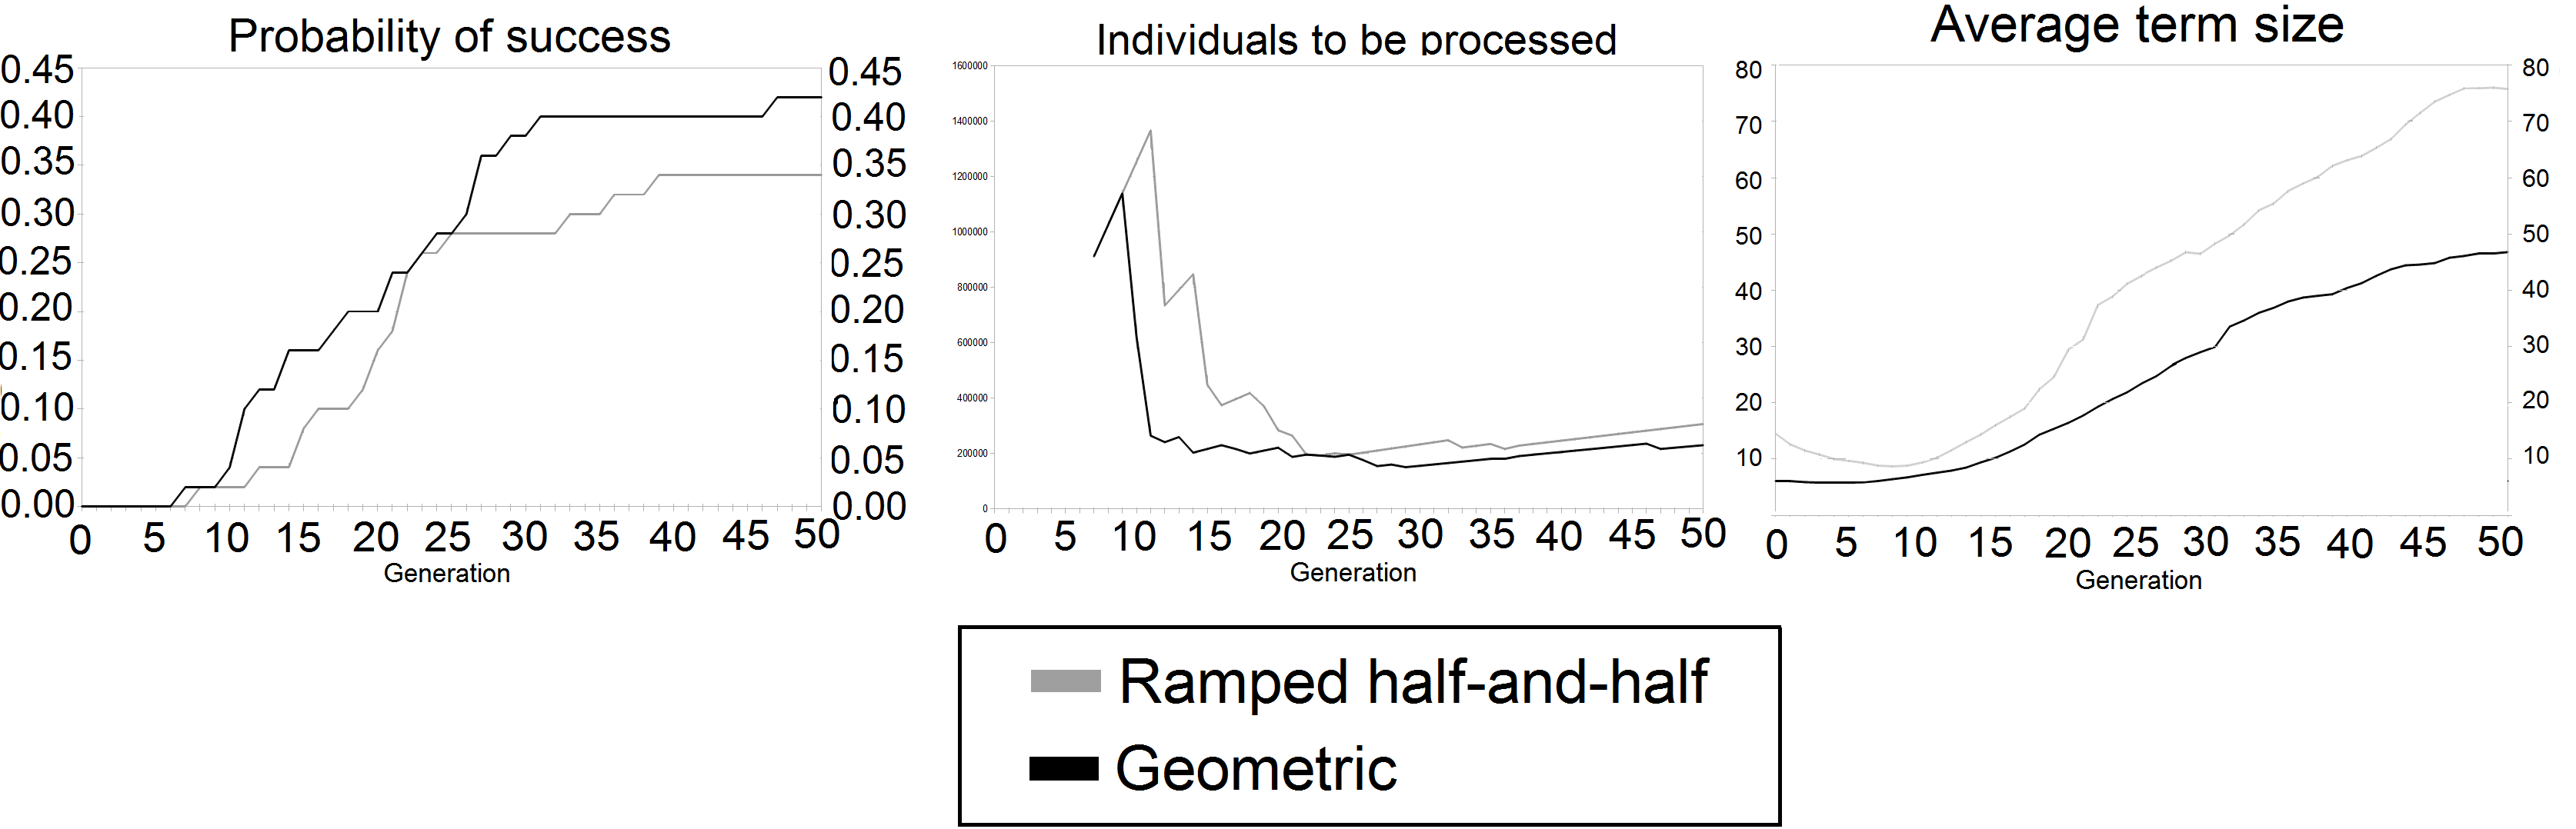
\includegraphics[scale=0.135]{imgs/SSR_FINAL.png}
\end{figure}
Fitness function is computed as follows.
$$ fitness(f) =  \sum\limits_{i=1}^{20}{ \vert f(x_i)-y_i }\vert   $$
where $(x_i,y_i)$ are 20 data samples from $[-1,1]$, such that $y_i = f_t(x_i)$.
An individual $f$ such that $\vert f(x_i)-y_i \vert < 0.01 $ for all data samples is 
considered as a correct individual.

Standard \textit{ramped half-and-half strategy} scored 17/50 (34\%) success rate. 
Minimal $I(M,i,z)$ was in generation 23 with 192,000 individuals to be processed.
The average individual size for generation 50 was 76.
The experiment took 46 minutes.
Our \textit{geometric strategy} scored 21/50 (42\%) success rate. 
Minimal $I(M,i,z)$ was in generation 29 with 150,000 individuals to be processed.
The average individual size for generation 50 was 47.
The experiment took 26 minutes.
Figure~1 shows the progress of those metrics throughout generations.
So for the \textit{Simple symbolic regression}
our geometric strategy is slightly more successful then 
ramped half-and-half strategy in all observed metrics.

\subsection{Artificial ant}
\textit{Artificial Ant} is another problem described
in \cite{koza92}. Objective of this problem is to 
find a control program for an artificial ant so
that it can find all food located on "Santa Fe" trail.
The Santa Fe trail lies on toroidal square grid.
The ant is in the upper left corner, facing right.
The ant is able to move forward, turn left, and sense if a food 
piece is ahead of him.

\begin{align*}
\tau = An&tAction\\
\Gamma = \{~~
  l    &: AntAction                              ,
  r    : AntAction                               ,
  m    : AntAction                               ,\\
  ifa  &: AntAction \ar AntAction \ar AntAction  ,\\
  p2   &: AntAction \ar AntAction \ar AntAction  ,\\
  p3   &: AntAction \ar AntAction \ar AntAction \ar AntAction  \}
\end{align*}

Action $l$ turns the ant left. 
Action $r$ turns the ant right.
Action $m$ moves the ant forward.
Action $ifa~x~y$ (if-food-ahead) performs action $x$ 
if a food piece is ahead of the ant,
otherwise it performs action $y$.
Action $p2~x~y$ first performs action $x$ and after it action $y$.
Action $p3~x~y~z$ first performs action $x$, 
after that action $y$ and finally $z$.
Actions $l, r$ and $m$ each take one time step to execute.
Ants action is performed over and over again until it reaches predefined
maximal number of steps. 

\begin{figure}[h!]
  \caption{Performance curves for Artificial ant problem.}
  \centering
    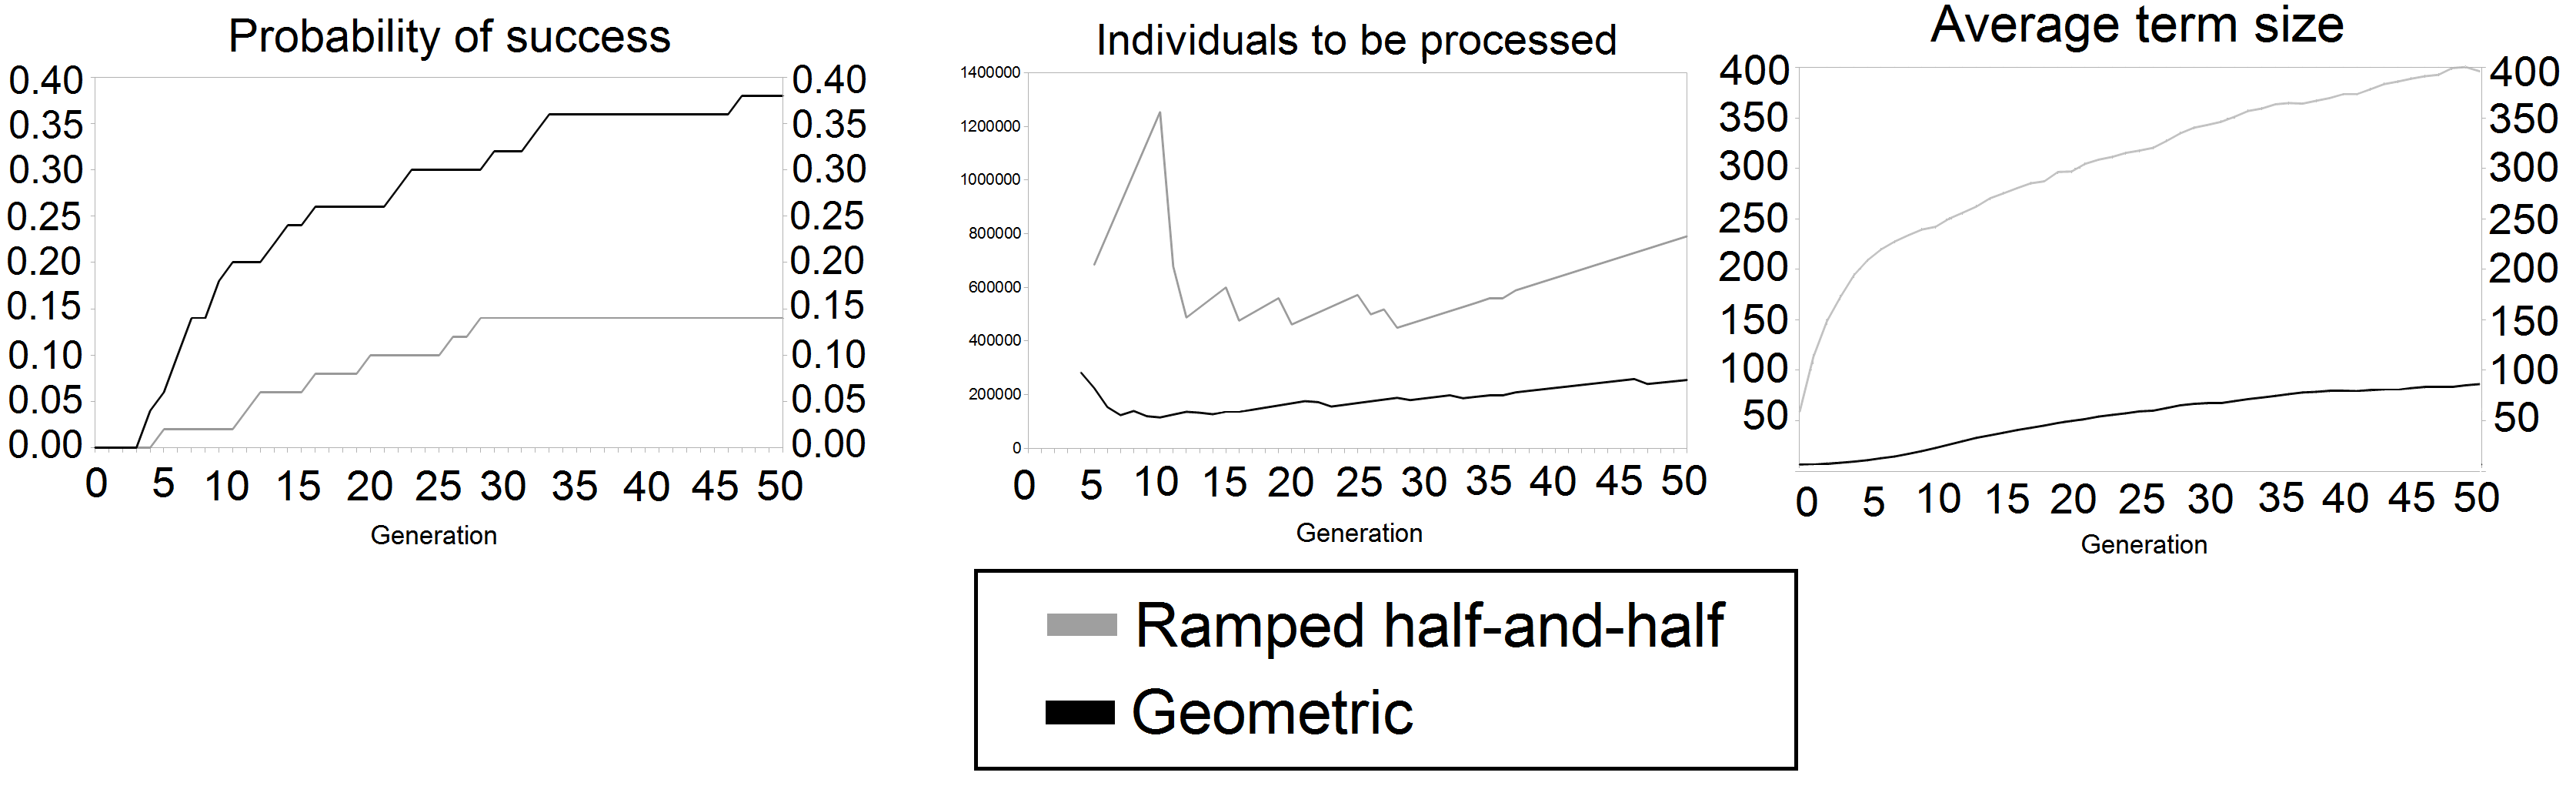
\includegraphics[scale=0.135]{imgs/ANT_FINAL.png}
\end{figure}

Fitness value is equal to number of eaten food pieces.
An individual such that eats all 89 pieces of food is 
considered as a correct solution.
This limit is set to be 600 time steps\footnote{
In \cite{koza92} this limit is said to be 400 time steps.
But there is also mentioned following solution, 
which is described as correct solution:
\texttt{(ifa m (p3 l (p2 (ifa m r) (p2 r (p2 l r)))(p2 (ifa m l) m)))}.
This program needs 545
time steps; if it is given only 400 time steps, then it eats only 79 pieces
of food. Thus we use 600 time steps. 
}.

Standard \textit{ramped half-and-half strategy} scored 7/50 (14\%) success rate. 
Minimal $I(M,i,z)$ was in generation 28 with 449,500 individuals to be processed.
The average individual size for generation 50 was circa 400.
The experiment took 265 minutes.
Our \textit{geometric strategy} scored 19/50 (38\%) success rate. 
Minimal $I(M,i,z)$ was in generation 10 with 115,500 individuals to be processed.
The average individual size for generation 50 was circa 90.
The experiment took 107 minutes.
This is a big improvement in all watched factors.
Figure~2 shows it in greater detail.

\subsection{Even parity problem}

Previous two problems were instances of standard GP, i.e. their building symbols
obeyed the closure requirement. This third experiment will break the closure requirement, thus ideal for testing typed GP techniques. 
The even-parity function is a boolean function taking as inputs $N$
boolean values and returning \textit{True} if an even number of inputs 
are \textit{True}. For odd number it returns \textit{False}.
This problem has been used by many researchers
as a benchmark for GP. We compare our results with that obtained by Yu in \cite{yu01},
where is presented approach to evolve recursive and modular programs
by use of higher-order functions and $\lambda$-abstractions.
We use very similar set of \textit{building symbols} as in \cite{yu01}. 
\begin{align*}
\tau = [Boo&l] \ar Bool\\
\Gamma = \{
  and   &: Bool \ar Bool \ar Bool                              ,
  or    : Bool \ar Bool \ar Bool                              ,\\
  nand  &: Bool \ar Bool \ar Bool                              ,
  nor    : Bool \ar Bool \ar Bool                              ,\\
  foldr &: (Bool \ar Bool \ar Bool) \ar Bool \ar [Bool] \ar Bool ,\\
  head' &: [Bool] \ar Bool                                   ,
  tail' : [Bool] \ar [Bool]                              \}
\end{align*}
\begin{figure}[h!]
  \caption{Performance curves for Even parity problem.}
  \centering
    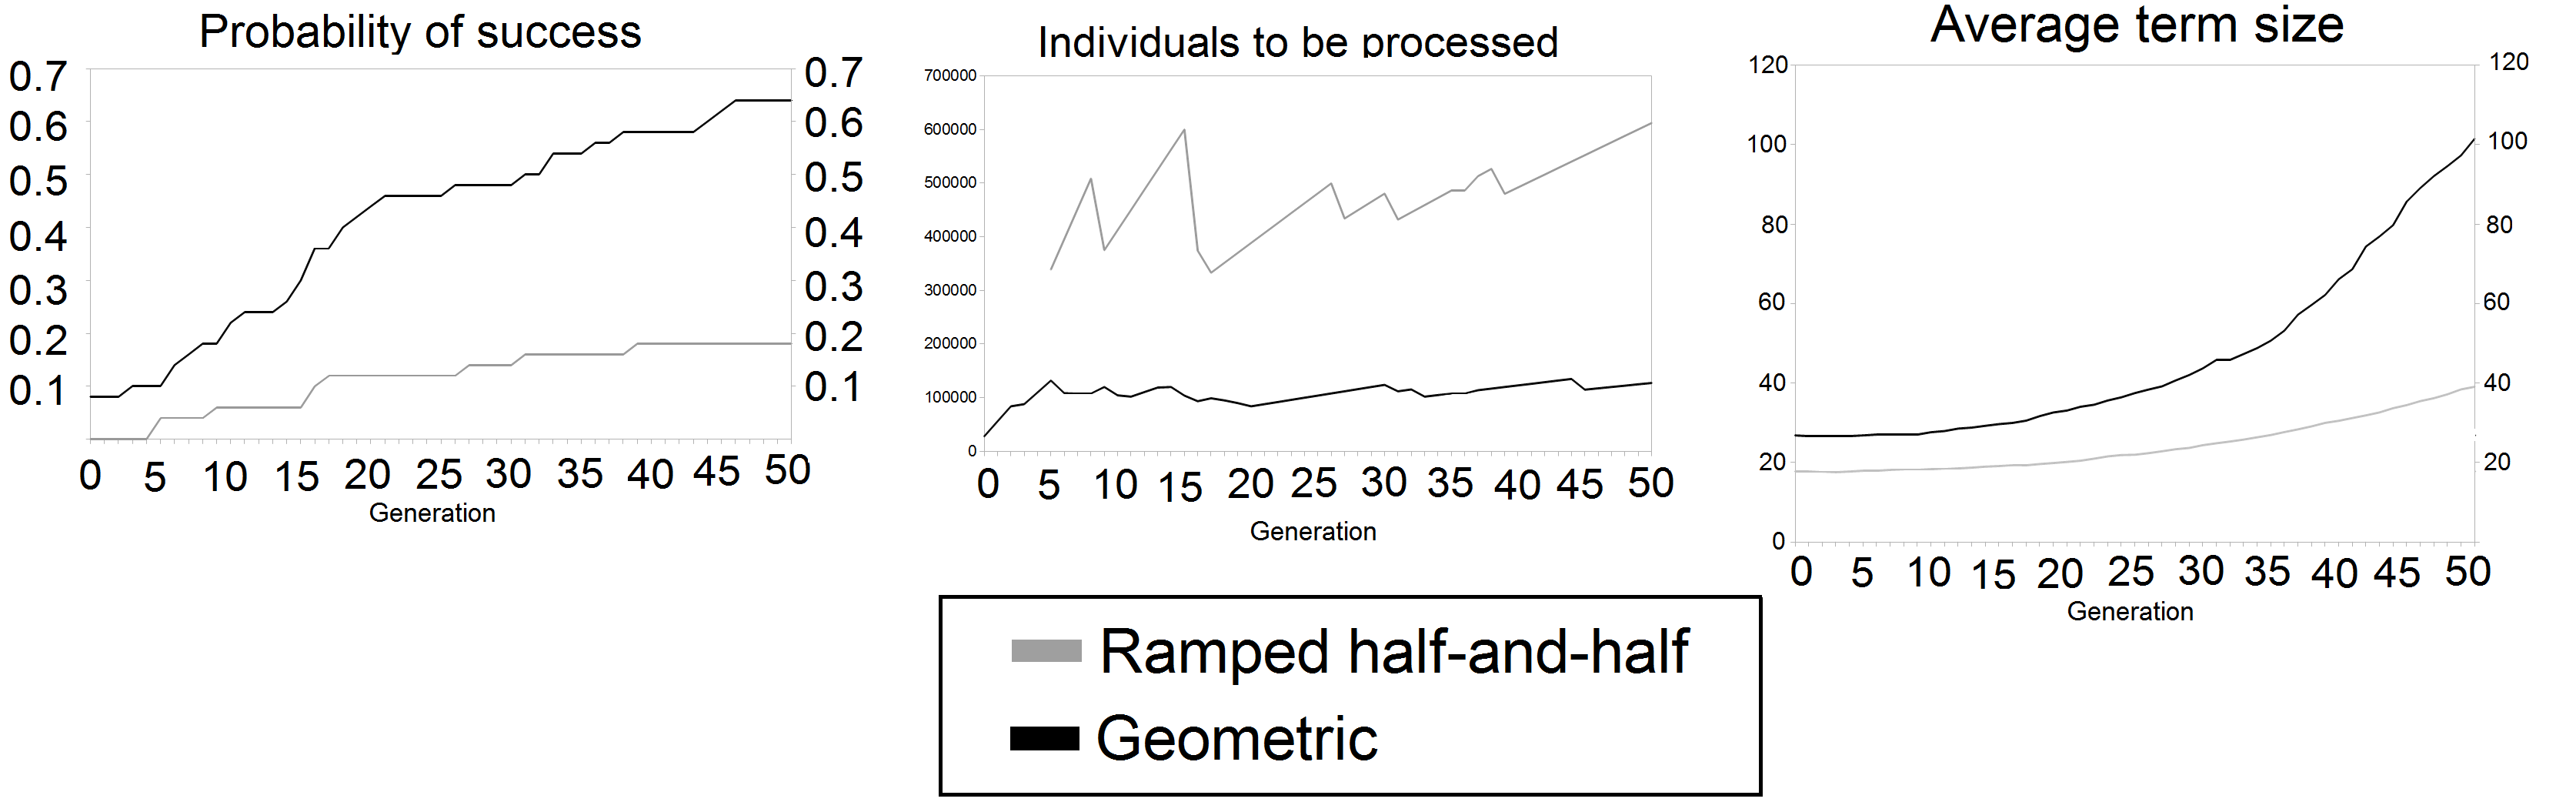
\includegraphics[scale=0.135]{imgs/EP_FINAL.png}
\end{figure}

The type $[Bool]$ stands for \textit{list of $Bool$s} and for purpose of
this problem is considered atomic.
Unlike in \cite{yu01}, we use specific instance of polymorphic 
function \texttt{foldr}. 
And modifications of functions \texttt{head} 
(returning the first element of the list) 
and \texttt{tail} (returning the list without the first element) are used; 
making them total by returning default value \textit{False}
and \texttt{[]}, respectively.
We use the same fitness function as in \cite{yu01}. 
The fitness function examines the individual by giving
it all possible boolean lists of length 2 and 3.

Standard \textit{ramped half-and-half strategy} scored 9/50 (18\%) success rate. 
Minimal $I(M,i,z)$ was in generation 17 with 333,000 individuals to be processed.
The average individual size for generation 50 was 39.
The experiment took 28 minutes.
Our \textit{geometric strategy} scored 32/50 (64\%) success rate. 
Minimal $I(M,i,z)$ was in generation 0 with 28,000 individuals to be processed.
The average individual size for generation 50 was circa 100.
The experiment took 33 minutes.
Figure~3 shows it in greater detail.
Once again this is a big improvement against standard method. 
One may get the impression that geometric strategy suffers from bloat here,
but considering that it performs significantly better and
that term size around 100 is similar as for the previous two problems, 
it seems to us that ramped half-and-half maybe has difficulties with 
constructing more complex terms, and therefore is "staying small".
Another remarkable observation is that 4 times out of 50 (8\% of all runs) 
the 100\% correct solution was present in the generation 0. This is pretty good
result for uninformed search. However, our results are less successful 
then those presented in \cite{yu01} (with slightly different set of 
building symbols); they scored 40/50 (80\%) success rate and $I(M,i,z)$ of 
17,500 in generation 4. But by observation of typical solution which is often
some modification of \texttt{foldr xor False inputList} one sees that important task
for GP here is to create \texttt{xor} function. This is advantage for the more specialized term representation used in \cite{yu01} 
(restricting use of outer variables). 
The difference in crossover operators may also be involved in the difference, 
but such analysis is beyond the scope of this paper. Finally, our result at least outperforms other results mentioned in \cite{yu01}: \textit{Generic genetic programming} 
scored 17/60 (28\%); min $I(M,i,z) = 220,000$. \textit{GP with ADFs} 
scored 10/29 (34\%); min $I(M,i,z) = 1,440,000$.


\section{Conclusions}
\label{conclusions}

In this work, we have proposed a generalization of genetic programming 
for simply typed lambda calculus. The main focus of this paper is on individual generation algorithms. 
The main idea is to explore the spectrum of available approaches bounded on one end by the traditional
ramped half-and-half strategy, while the second bound represents an exhaustive systematic search. 
Thus, three population initialization methods have been designed, 
depending on different search strategies. 
The first strategy corresponds to the above mentioned traditional genetic programming initialization,  
the second one corresponds to exhaustive search, and the third one 
represents a novel geometric strategy which outperforms standard genetic 
programming in success rate, resource consumption and average individual size 
on the presented experiments. 

%\red{ [větu dvě o experimentech]}

The relevance of these algorithms does not effect only initialization, but it can be used during mutation
operator in a straightforward way. 
%Other performance enhancements based on theory of lambda calculus are 
%proposed and supported by experiments, including abstraction 
%elimination that enables us to utilize
%a simple tree-swapping crossover.

Our future research will focus on exploring other possible search strategies positioned in the middle ground 
identified in this paper. Since the search strategy can be easily described by a rather simple filtration algorithm, it might be
interesting to allow the typed GP system to evolve the search strategy it 
utilizes in a kind of meta-evolution way. 

%\red{ [ještě něco navíc nebo podrobněji, říct poly že neni ale že se na něm pracuje a de hezky zandat do již systemu] }


\nocite{*}

\bibliographystyle{splncs}
\bibliography{evogp}


\end{document}


%
%\begin{thebibliography}{1}
%
%
%\bibitem{koza92}
  %John R. Koza,
  %\emph{Genetic Programming: On the Programming of Computers by Means of Natural Selection}.
  %MIT Press, Cambridge, MA,
  %1992. 
%
%\bibitem{koza05}
  %Koza, J.R., Keane, M., Streeter, M., Mydlowec, W.,Yu, J., Lanza, G. 
  %\emph{Genetic Programming IV: Routine Human-Competitive Machine Intelligence.} 
  %Springer, 2005. ISBN 978-0-387-26417-2 
%
%\bibitem{fg}
 %Riccardo Poli, William B. Langdon, Nicholas F. McPhee
 %\emph{A Field Guide to Genetic Programming}.
 %Lulu Enterprises, UK Ltd, 2008.
%
%\bibitem{yu01}
  %T. Yu. 
  %\emph{Hierachical processing for evolving recursive and modular 
        %programs using higher order functions and lambda abstractions}. 
  %Genetic Programming and Evolvable Machines,
  %2(4):345–380, December 2001. ISSN 1389-2576.
%
%
%\bibitem{montana95}
%D. J. Montana. 
%\emph{Strongly typed genetic programming.} 
%Evolutionary Computation, 3(2): 199–230, 1995.
%%URL \url{ http://vishnu.bbn.com/papers/stgp.pdf }. nefacha
%
%\bibitem{haynes96}
%T. D. Haynes, D. A. Schoenefeld, and R. L. Wainwright. 
%\emph{Type inheritance in strongly typed genetic programming.} 
%In P. J. Angeline and K. E. Kinnear, Jr., editors, Advances
%in Genetic Programming 2, chapter 18, pages 359–376.
%MIT Press, Cambridge, MA, USA, 1996. ISBN 0-262-01158-1. 
%%URL \url{http://www.mcs.utulsa.edu/~rogerw/papers/Haynes-hier.pdf}.
%
%\bibitem{olsson94}
%J. R. Olsson. 
%\emph{Inductive functional programming using incremental program 
%transformation and Execution of logic programs by 
%iterative-deepening A* SLD-tree search.} 
%Dr scient thesis, University of Oslo, Norway, 1994.
%
%\bibitem{kes}
%Forrest Briggs, Melissa O’Neill.
%\emph{Functional Genetic Programming and Exhaustive
%Program Search with Combinator Expressions.}
%International Journal of Knowledge-based and Intelligent Engineering Systems,
%Volume 12 Issue 1, Pages 47-68, January 2008. 
%
%
%\bibitem{barendregt84}
%H. P. Barendregt,
%\emph{The Lambda Calculus: its Syntax and Semantics}, 
%revised ed., North-Holland, 1984.
%
%\bibitem{barendregt92}
%H. Barendregt , S. Abramsky , D. M. Gabbay , T. S. E. Maibaum.
%\emph{Lambda Calculi with Types.} 
%Handbook of Logic in Computer Science, 1992. 
%
%\bibitem{barendregt10}
%
  %Henk Barendregt, Wil Dekkers, Richard Statman,
  %\emph{Lambda Calculus With Types}.
  %Cambridge University Press,
  %2010. 
  %%URL \url{http://www.cs.ru.nl/~henk/book.pdf}.
%
%\bibitem{jones87}
%Simon Peyton Jones. 
%\emph{The Implementation of Functional Programming Languages}. 
%Prentice Hall, 1987.
%
%
%\bibitem{AIAMA}
	%Stuart J. Russell, Peter Norvig,
	%\emph{Artificial Intelligence: A Modern Approach}.
	%Pearson Education,
	%2003. 
%
%
%\end{thebibliography}

